\newpage
\section{Aufbau und Funktionsweise der Messaperatur}

	\begin{wrapfigure}{r}{0.6\textwidth}
		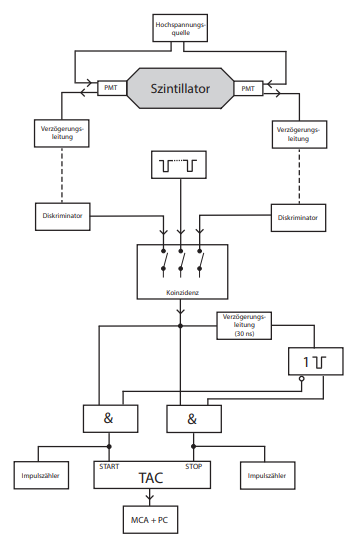
\includegraphics[width=10cm]{latex/images/Aufbau.png}
		\caption{Skizze der Schaltung \cite{V01}}
		\label{fig:Aufb}
	\end{wrapfigure}
    In Abbildung \ref{fig:Aufb} ist die in diesem Versuch verwendete Schaltung gezeigt.
    Diese Schaltung wird genutzt um zu erkennen wie viele Myonen in dem Messzeitraum in den Messkörper eintreten, wie viele dieser eingetreten Myonen innerhalb des Körpers zerfallen und wie viel Zeit zwischen dem Einfall und Zerfall liegt.
    Der Messkörper ist ein organischer Szintillationstank mit einem Volumen von ungefähr 50 Litern.\\
    Beim Eintreten der Myonen in den Detektor werden die Myonen abgebremst und erzeugen einen Lichtblitz.
    Zerfällt das Myon innerhalb des Detektors entsteht ein hochenergetisches Elektron welches wiederum wieder mit dem Szintillatormaterial wechselwirkt und einen Lichtblitz erzeugt.
    Zur Messung dieser Signale sind an beiden Enden des Tanks Photomultiplier(englisch: \textit{photomultiplier tube} (PMT)) angebracht. Diese wandeln das eingehende Lichtsignal in einen Spannungsimpuls um. \\
    Der PMT ist über eine Verzögerungsleitung an Diskriminatoren angeschlossen.
    Die Diskriminatoren dienen dazu den Großteil der thermischen Anregungen der PMTs auszufiltern, welche niederenergetischer sind als die Myonen Signale.
    An den Diskriminatoren wird eine gewisse Schwellspannung $U_0$ eingestellt, damit möglichst viele Rauschsignale unterdrückt werden aber auch möglichst keine echten Signale verloren gehen.
    Des Weiteren werden höherenergetische thermische Anregungen der PMT ausgefiltert, indem beide Diskriminatoren an eine Koinzidenzschaltung angeschlossen werden.
    Die Koinzidenzschaltung gibt nur ein Signal weiter, wenn beiden eingehenden Signale innerhalb eines Zeitraumes $t_\text{k}$ eintreffen.
    Mit diesen beiden Filtermethoden können der unkorrelierte Untergrund nur mit einer sehr geringen Wahrscheinlichkeit ein Signal erzeugen.\\
    Jetzt folgt der Schaltungsteil der zählt, wie viele Signale entstehen und falls das Myon innerhalb des Detektors zerfällt, wie lange es gelebt hat.
    Dies erfolgt, indem das Outputsignal der Koinzidenzschaltung in 3 Signale aufgeteilt wird.
    Zwei dieser Signale werden jeweils an eine Seite eines AND-Gatters angeschlossen. 
    Das Dritte wird mit einer Verzögerung von $\SI{30}{\nano\second}$ an einen Monoflop angeschlossen.\\
    Der Monoflop gibt nach dem er durch ein HIGH-Signal getriggert wurde für eine gewisse einstellbare Zeit $T_\text{S}$ ein HIGH Signal aus. 
    Dies ist die Suchzeit $T_\text{S}$ in der ein weiters Signal als ein zerfallenes Myon interpretiert wird.
    Der Output des Monoflops ist nun invertiert an dem 1. AND-Gatter und normal an dem 2. AND-Gatter angeschlossen.
    Wenn die Schaltung im Ruhezustand ist und das Signal eines eintretenden Myon ankommt, 
    liegen an dem ersten AND-Gatter nun zwei HIGH-Signale an, da durch die Verzögerung der Monoflop noch nicht aktiviert wurde.
    Dieses HIGH-Signal wird an einen Impulszähler weitergegeben und startet zudem den Zeit-Amplituden-Converter(TAC).
    Am zweiten AND-Gatter liegen aufgrund der Verzögerung ein HIGH und LOW-Signal, es entsteht also kein Signal für den Zerfall eines Teilchens.\\
    Wenn das Myon jetzt jedoch innerhalb der Suchzeit $T_\text{S}$ zerfallen ist und ein weiteres Signal erzeugt verhält sich die Schaltung anders.
    Jetzt liegt durch den Monoflop noch ein LOW-Signal am ersten AND-Gatter an.
    Der erste Impulszähler und der Zeit-Amplituden-Converter werden nicht erneut aktiviert.
    An dem zweiten AND-Gatter liegen dann jedoch zwei HIGH-Signale an. Dieses ist an einen Impulszähler und an den TAC angeschlossen und stoppt diesen.
    Der Zeit-Amplituden-Converter gibt nun ein Signal mit einer Spannungshöhe korreliert zu der Zeit zwischen den Signalen an einen Multi-Channel-Analyser(MCA) weiter.
    Dieser wird von einem PC ausgewertet.

\section{Durchführung}
	
	Zunächst wird die Schaltung nach Abbildung \ref{fig:Aufb} aufgebaut. 
    Dazu müssen die verschiedenen Schaltungskomponenten korrekt aneinander geschaltet werden.\\
	Dann folgt die Justierung der Schaltung. Dabei wird neben den Messgeräten des Versuches ein Oszilloskop verwendet.
	Zunächst werden die Schwellspannungen an den Diskriminatoren so eingestellt, dass auf beiden Seiten eine Signalrate von ca. $\SI{30}{\hertz}$ vorliegt. 
    Dann werden die Einstellungen der Verzögerungsleiter bei einer Pulsdauer von $\Delta t= \SI{20}{\nano\second}$ und $\Delta t= \SI{10}{\nano\second}$ variiert.
	Die Pulsdauern werden an den Diskriminatoren über kleine Schrauben verändert und an dem Oszilloskop abgelesen.
	Es werden beide Diskriminatoren an die Koinzidenzschaltung geschaltet und je einer der Verzögerungsleiter verstellt und die Signalrate gemessen.
	Durch systematisches, einzelnes Verstellen der Verzögerungen ergibt sich eine Kurve der Signalraten. 
    Dabei sollten genug Werte aufgenommen werden, um die Halbwertsbreite dieser Kurve zu bestimmen.\\
	Jetzt wird für den restlichen Versuch bei einer Signallänge von $\Delta t= \SI{10}{\nano\second}$ die optimale Verzögerung eingestellt.
    Es sollte eine Ereignisrate im Bereich von $\SI{20}{\hertz}$ anliegen, dazu wird an dem Monoflop eine Suchzeit von $T_\text{S} = \SI{10}{\micro\second}$ eingestellt.\\
	Des Weiteren wird der TAC so eingestellt, dass möglichst viele Kanäle des MCA genutzt werden.
	Dafür wird der Doppelpulsgenerator mit einem Impulsabstand von $\SI{10}{\nano\second}$ an die Koinzidenzschaltung geschaltet und der TAC so eingestellt, dass ein Channel in der Mitte angesprochen wird.\\
	Zuletzt werden noch der TAC und der MCA so kalibriert, dass aus der Spannungshöhe bzw. dem Channel eine Lebensdauer berechnet werden kann.
	Dazu wird wieder der Doppelpulsgenerator an die Koinzidenzschaltung angeschlossen, 10 unterschiedliche Impulsabstände eingestellt und jeweils der damit korrespondierende Kanal ausgelesen.
	Mit den Informationen der Channel und der Impulsabstände lässt sich der TAC und der MCA kalibrieren.\\
    Zuletzt wird die Messung der Lebensdauern der Myonen gestartet. 
    Dafür werden über einen Zeitraum von ungefähr zwei Tagen die Lebensdauern der Myonen am Computer und die Startsignale an einem der Zähler aufgenommen.
